\section{Background}
This section presents a review of existing algorithms, an anomaly taxonomy, and evaluation of existing anomaly detection libraries. Additionally, this section includes an overview of the Work Packages (WPs) that define the deliverables of the FIREMAN project.

\subsection{FIREMAN Work Packages}
\label{ref_FIREMAN_WP}

This subsection outlines the progress and overall goal of the three milestones or work packages that guide the FIREMAN project. The interconnection and overview of the individual WPs is shown in Figure \ref{fig:wp-diagram}

\begin{figure}[H]
    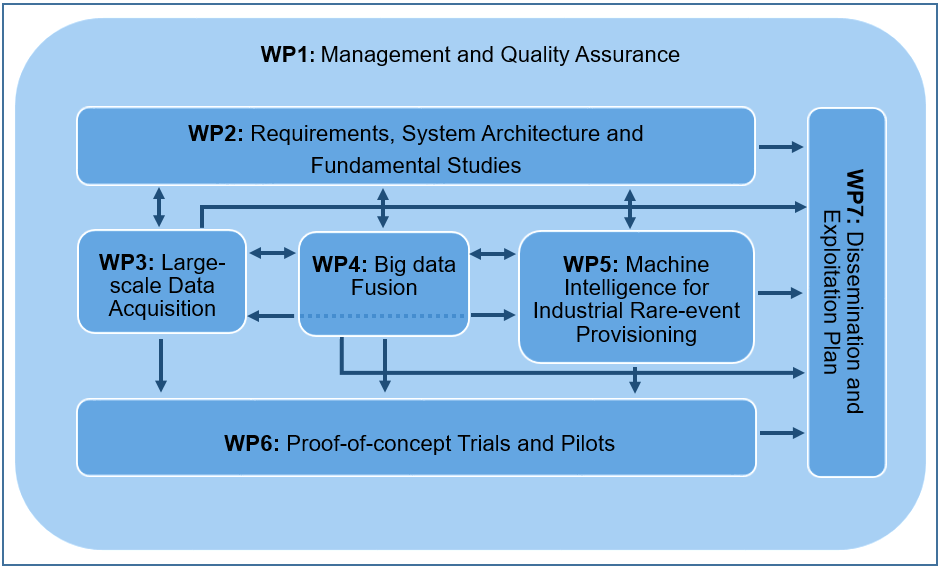
\includegraphics[width=\textwidth]{Images/FIREMAN_pert_diagram.png}
    \caption{FIREMAN WP Diagram \parencite{fireman-homepage}}
    \label{fig:wp-diagram}
\end{figure}

This work focuses on Proof-of-Concept Trails and Pilots (WP6) by demonstrating an implementation of a theoretical algorithm for real-world anomaly detection.

\subsubsection{Large Scale Data Acquisition (WP3)}

This work package focuses on \enquote{event-based modelling and traffic characterization techniques aiming for a reduced use of communication and storage resources. This pre-processing task is expected -among others- to optimize the subsequent data transmissions by injecting only relevant data in the network to reduce overhead and increase spectral efficiency.} \citel{wp3.1}

In this portion of FIREMAN, we examined a  variety of industrial datasets including the Tennessee Eastman Process, Electricity Metering, IEC-61850 Distribution Automation, and the EPFL Smart Grid Pilot. This dataset is not heavily reliant on relational constraints or atomicity, consistency, isolation, durability (ACID) compliance. Because of this, we have selected a non-relational PostgreSQL database for storage because of its superior throughput and increased performance in data processing applications.

The sensors traditionally used in Cyber-Physical Systems do not have much compute or storage capacity which makes pre-processing of data at the sensor level challenging. Because of this, \enquote{compression is essential for reducing the challenge of data storage, collection, transmission, processing, and analysis at the local level}\parencite{compression}. Authors \cite{wp3.2} have shown that it is possible to achieve a 92.6\% compression rate which means that only 7.4\% of samples are transmitted. We have also used different methods including linear interpolation to de-compress the data and have measured the error using the root mean square technique. 

% \begin{figure}[H]
%     % \centering
%     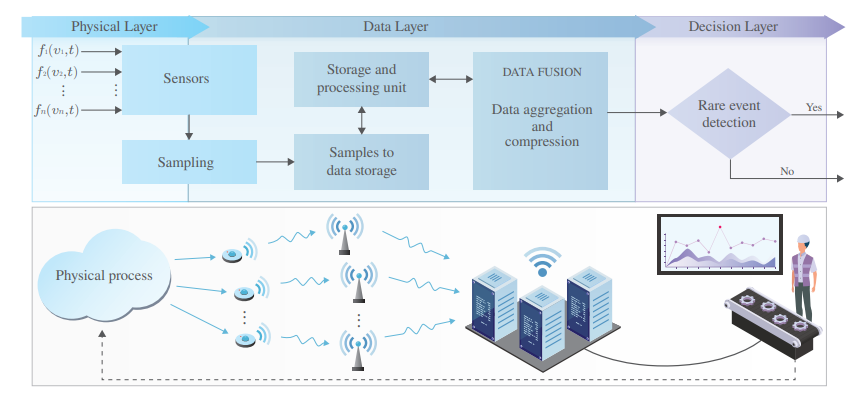
\includegraphics[width=\textwidth]{Images/three-layer-system.PNG}
%     \caption{Three layer framework for rare event detection \parencite{three-layer-approach}}
%     \label{fig:three-layer}
% \end{figure}

Modeling of transmission reduction techniques centered around the electricity modeling dataset \parencite{elect-model-dataset-9694611}. Three approaches for reducing transmissions were presented including transmission on large spikes, transmissions on accumulated variance, and time interval defined transmission with a timeout to compensate for meter or network failure. These simulations have shown a large potential for reducing transmissions without significantly affecting the accuracy of the measured signal. We modeled a Markov-Modulated Poission Process to simulate these industrial processes for use in further stages of the project.

\subsubsection{Big Data Fusion (WP4)}
\label{ref_wp4}
The goal of this task is \enquote{to show how a large number of sensors and their corresponding data can be  accommodated and aggregated at small cost for reliably detecting rare events}\parencite{wp4.1}. This task focuses on three primary objects: 
\begin{inlinelist}
    \item heterogeneous data aggregation in machine-type communications;
    \item signature-based cluster formation; and
    \item IoT platform and database selection.
\end{inlinelist}

It is challenging to simultaneously connect a massive number of devices which is why data aggregation is important.
This strategy outlined by Authors \cite{massive-machine} relies on the following principals:
\begin{inlinelist}
  \item decreasing communication distance and power consumption of connected devices;
  \item utilizing an efficient distributed node routing network to decrease bandwidth congestion of central nodes; and
  \item extending the network coverage.
\end{inlinelist}
The researchers also introduced a cluster formation scheme based on signatures that reduces the signalling overhead required for peer-discovery in the network. This technique utilizes signal aggregates to reduce traffic congestion to the central node.

Additionally we surveyed IoT experts to determine the most important properties and components of an IoT system. This survey compared the five most popular cloud IoT providers: AWS, Azure, GCP, IBM Watson, and Oracle IoT to create a comparison that can be used by businesses when selecting a cloud provider that suits their business needs \parencite{choose-iot-9110590}.

SEAT, an automotive component manufacturer, provided two use cases and accompanying datasets for the FIREMAN project. The first involves early failure detection of mechanical components in the drive chain in the Paint shop which causes axial displacement. The second involves detecting early failure of the spindle on a CNC machine which ensures lineal movement over a surface. In both of these situations detecting failure early helps SEAT detect problems and solve them before they begin to impact production components and eventually reduce production downtime to zero. 

\subsubsection{Machine Intelligence for Industrial Rare-event Provisioning (WP5)}

The goal of this task is to utilize machine intelligence techniques to predict indicators of health for a machine, component, or entire industrial process to determine health and detect premature failure. The main technique proposed in this task is Quantitative Association Rule Mining Algorithm (QARMA).

\enquote{QARMA is a family of algorithms for extracting all (or, depending on user inputs, an important subset of) valid non-dominated quantitative association rules that hold in a dataset, that can then be used for further data analysis such as deriving rule-based classifier ensembles or as explainers of classification results of other black-box classifiers.}\citel{wp5.1}  This technique is one of the most human understandable techniques for machine intelligence and has shown promise for this application. In this WP, QARMA is tested on the SEAT dataset discussed in \ref{ref_wp4}.

Traditional methods for pruning the rules created by the algorithm were analyzed in this WP as many of them can be extraneous or unreliable. The fastest open source Mixed-Integer Programming (MIP) tool was able to solve this problem in 19 seconds while the parallelized hybrid search algorithm proposed in this WP solved the problem 240 times faster when using parallel threads.

Authors \cite{wp5.1} used a breadth first search approach to compute a `small' subset of rules that cover the majority of instances in a training dataset covered by the totality of rules extracted by QARMA applied on it. Through experimentation on a synthetic power grid fault diagnostic dataset QARMA performs better than certain neural networks with noisy data \parencite{ml-performance-power-trans}. This is because of the over-fitting of training data with Deep Neural Network architectures. The rule based methods generated by QARMA produce human understandable rules which is beneficial in creating explainable AI.

\subsubsection{Proof-of-Concept Trails and Pilots (WP6)}
\label{ref_wp6}

% TODO

\subsection{Algorithm Explainability}

Certain high-risk use cases for machine learning algorithms demand a high level of explainability and confidence in the algorithm outputs to use in fields of decision making. In many cases an algorithm makes a classification decision but there is not a clear explanation as to why the algorithm made that decision. In the field of power electronics, understanding why a data-driven controller is making a decision is critical to incorporating it into real world power distribution scenarios. 

Answering these questions is complex and there are a few approaches to achieving this goal. Authors \cite{black-box-explainability} propose using conditional entropy to determine how each input is related to each output. The generated plots are then compared to the physical insights of the system and outlier, adversarial data that falls outside the plot is identified and removed. The model is then retrained. This technique is helpful for identifying and removing adversarial data that falls outside the range of accepted values but it would not identify data overloading in a specific portion of the graph which would create an incorrect classification.

\subsubsection{Types of Uncertainty}
It is often necessary to determine sources of uncertainty in a model or system. When analyzing uncertainty, it is important to understand the two types:
\begin{inlinelist}
    \item epistemic and
    \item aleatoric uncertainty.
\end{inlinelist}

Epistemic uncertainty results from inadequate training data. With this type, the training data is not sufficient to provide enough or accurate date to the model. This can be a result of unbalanced or lack of training data. Increasing the amount of training data or decreasing class imbalance can help reduce this type of uncertainty. 

Aleatoric uncertainty arise from probabilistic errors in sampling that follow a specific probability distribution. This type of uncertainty is independent to the amount of data collected and therefore cannot be corrected with more training data. If a signal has noise inline with a given probability distribution, having more data on that signal does not change the noise probability distribution. This type of uncertainty references the distribution of random errors in the data and not the data distribution itself.

For illustration, suppose someone is recording audio at a train station. There are three announcements each hour that disrupt the recording but you do not know when in the hour they occur. Having more data (hours), does not change the amount of announcements that occur. 

\subsubsection{Combating Model Uncertainty}

With deep learning algorithms, it is important to know the level of confidence the model is predicting the outcome with. Authors \cite{explaining-adversarial-examples} explain that adding simple adversarial data (like small noise to a photo) makes an image recognition algorithm incorrectly classify one animal as a completely different one. This is further concerning since adversarial data does not need to be tailored to a specific algorithm. The transferability of this type of adversarial data allows it to be applied to many black box algorithms to achieve an unintended or potentially malicious result. 

A malfunctioning sensor or bad connection can generate noise (a type of aleatoric uncertainty), which cannot be fixed by more measurements or more data. Data imputation can be used as a technique to correct for or understand this type of uncertainty. If you can identify that the uncertainty is present, then you can use data imputation to form a well educated guess as to what the value should actually be. The significance of identifying it as aleatoric uncertainty is that no amount of model tuning or data collection can fix the underlying issue, so data imputation presents an opportunity to move forward that standard techniques would not.

Bayseaian techniques can be used to create a probability distribution over the weights to determine a level of uncertainty for the weights. Unfortunately, retraining a large number of models on a variety of datasets is computationally expensive and time consuming. Authors \cite{gal2016dropout} proposed using a dropout technique to approximate the Bayseaian representation. This technique avoids over-fitting by randomly sampling and dropping network nodes across many different training iterations.

It is important to perform the dropout technique while training and testing the algorithm and then compute the variance to determine the uncertainty. This enables researchers to determine that for specific values the algorithm is providing a best guess answer with high levels of uncertainty, which could then signal the need for human intervention or review in decision making.  

\subsection{Outlier Taxonomy}

The term `outlier' or `anomaly' can have a variety of interpretations and meanings depending on the context. In order to select and evaluate appropriate techniques for outlier detection, it is essential to understand and define the various types of outliers that can be present in a dataset. There are three ways that outliers are usually categorized in the literature:
\begin{inlinelist}
    \item contextual
    \item point and
    \item collective.
\end{inlinelist}
These three types of outliers are illustrated graphically in Figure \ref{fig:outliers-graphic}.

\begin{figure}[H]
    % \centering
    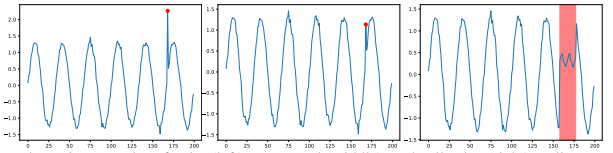
\includegraphics[width=\textwidth]{Images/outliers_graphic.PNG}
    \caption{[Point, Contextual, and Collective] Outliers \parencite{lai2021revisiting}}
    \label{fig:outliers-graphic}
\end{figure}

\begin{figure}[H]
     \centering
     \begin{subfigure}[b]{0.3\textwidth}
         \centering
         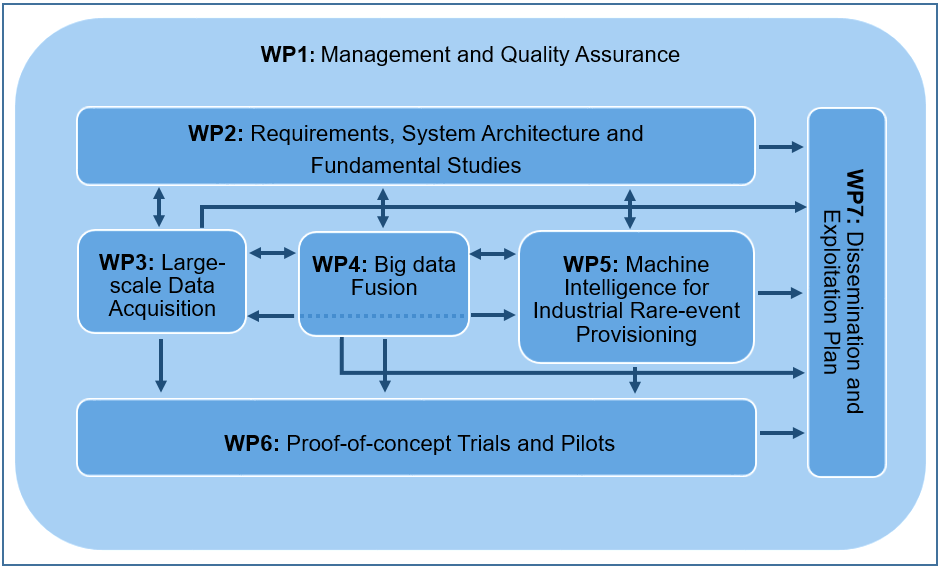
\includegraphics[width=\textwidth]{Images/FIREMAN_pert_diagram.png}
         \caption{Point Outlier}
         \label{fig:shaplet}
     \end{subfigure}
     \hfill
     \begin{subfigure}[b]{0.3\textwidth}
         \centering
         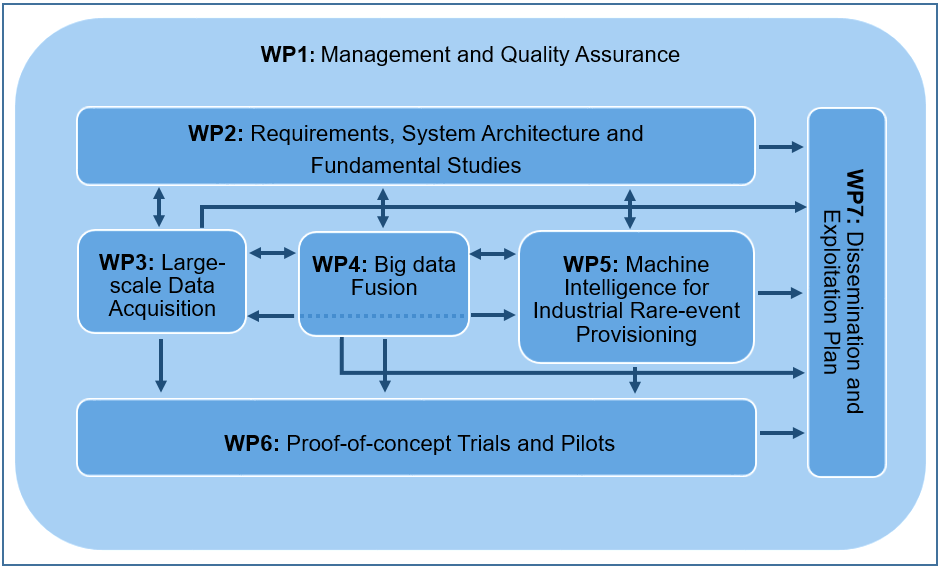
\includegraphics[width=\textwidth]{Images/FIREMAN_pert_diagram.png}
         \caption{Contextual Outlier}
         \label{fig:seasonal}
     \end{subfigure}
     \hfill
     \begin{subfigure}[b]{0.3\textwidth}
         \centering
         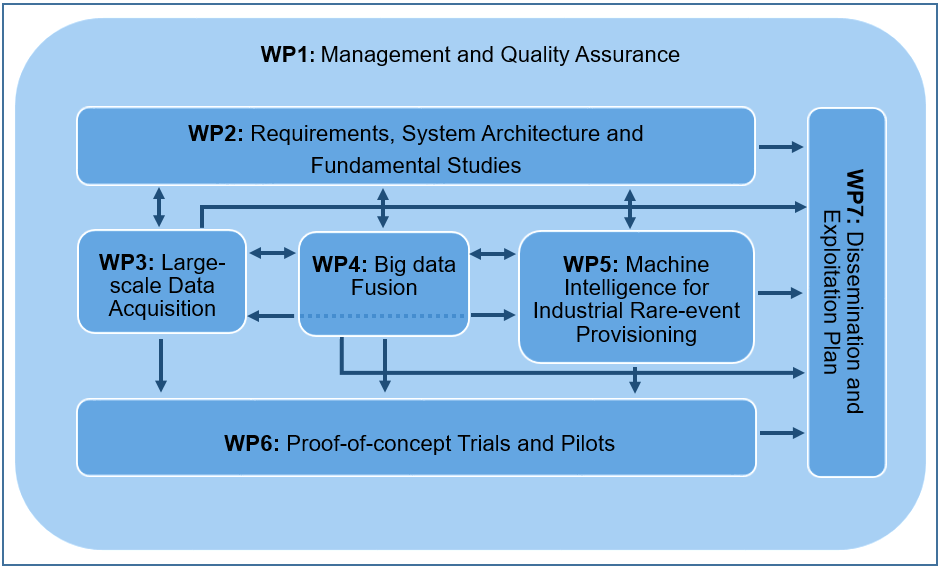
\includegraphics[width=\textwidth]{Images/FIREMAN_pert_diagram.png}
         \caption{Collective Outlier}
         \label{fig:trend}
     \end{subfigure}
        \caption{Outlier Taxonomy Adapted from \cite{lai2021revisiting}}
        \label{fig:outliers-graphic}
\end{figure}


Point outliers are single points that are anomalous in respect to the global dataset. This can cause many problems in machine learning algorithms and a large body of outlier detection research is focused around this area.These outliers can be non-temporal or temporal in nature and often represent phenomenon like intermittent sensor failure. 

Additionally, these types of outliers can skew scaling and normalization operations. It is important to consider the presence of these types of outliers when selecting which type of scaler to use. Minimum-Maximum scaling is a popular choice for scaling a dataset but it is not robust to outliers. 

Contextual outliers are points that are anomalous in respect to a specific sub-set or window of the dataset. An example would be an outlier point in a sinusoidal pattern. his represents a phenomenon that is anomalous with respect to a specific sub-window or pattern but it is not anomalous with respect to the global dataset. 

Collective or pattern-wise outliers are a subset of points that form an anomalous pattern in the context of the global dataset. Singular points within the collective outlier sub-set are usually not anomalous but the entire pattern is. These outliers occur often in time-series data because of the interdependence of samples and sampling time. This outlier type is the focus of the detector developed in this work.

\subsubsection{Collective Outliers}

Since collective outliers are the focus of this study, it is possible to further classify this outlier type into three sub-categories:
\begin{inlinelist}
    \item shaplet
    \item seasonal
    \item and trend outliers.
\end{inlinelist}
This subset of anomalies represents various anomalous sub-sequences of the data in a given context. Figure \ref{fig:contextual-outliers} represents these phenomenon graphically. 

\begin{figure}[H]
     \centering
     \begin{subfigure}[b]{0.3\textwidth}
         \centering
         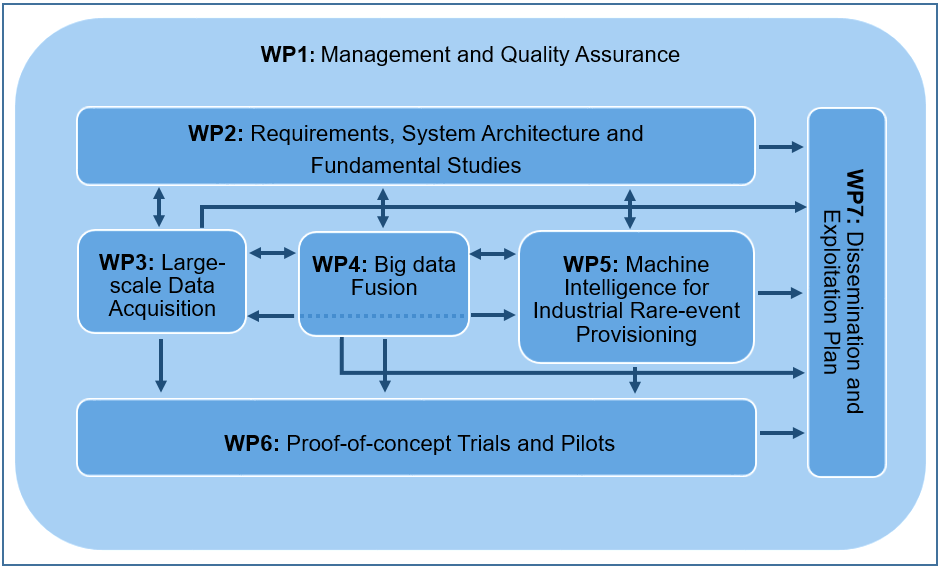
\includegraphics[width=\textwidth]{Images/FIREMAN_pert_diagram.png}
         \caption{Shaplet Outlier}
         \label{fig:shaplet}
     \end{subfigure}
     \hfill
     \begin{subfigure}[b]{0.3\textwidth}
         \centering
         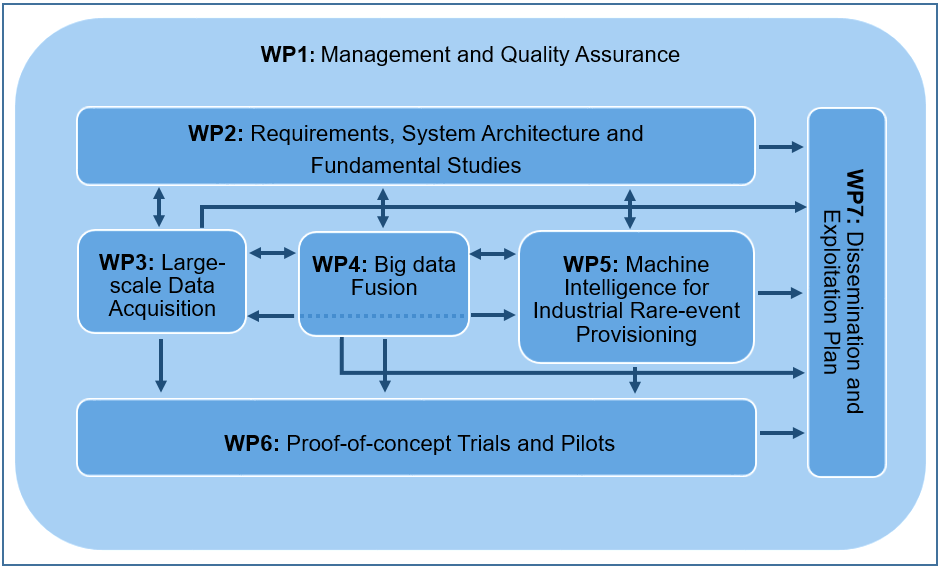
\includegraphics[width=\textwidth]{Images/FIREMAN_pert_diagram.png}
         \caption{Seasonal Outlier}
         \label{fig:seasonal}
     \end{subfigure}
     \hfill
     \begin{subfigure}[b]{0.3\textwidth}
         \centering
         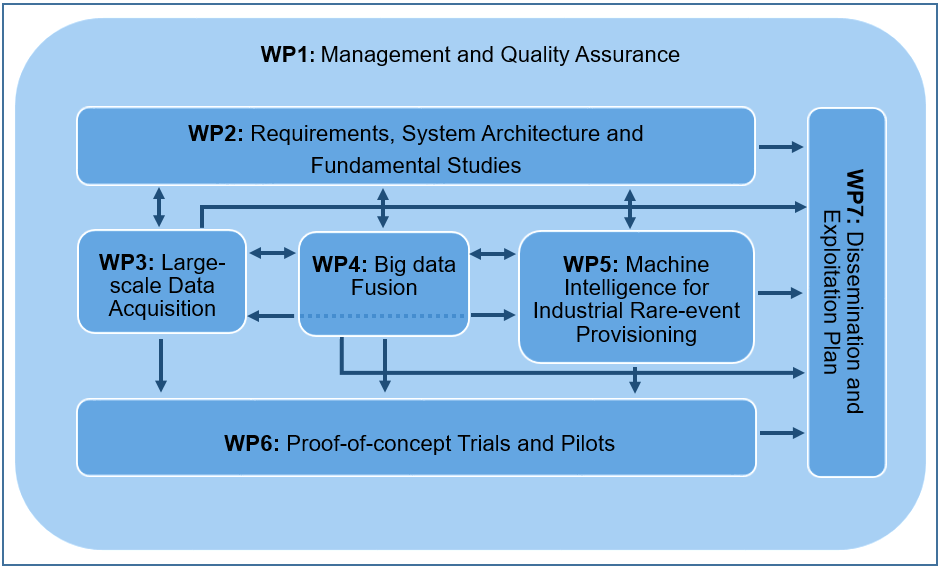
\includegraphics[width=\textwidth]{Images/FIREMAN_pert_diagram.png}
         \caption{Trend Outlier}
         \label{fig:trend}
     \end{subfigure}
        \caption{Collective Outliers Adapted from \cite{lai2021revisiting}}
        \label{fig:contextual-outliers}
\end{figure}

\begin{figure}[H]
    % \centering
    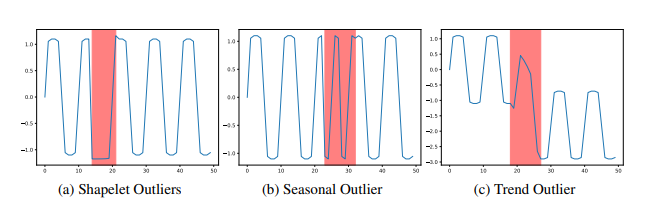
\includegraphics[width=\textwidth]{Images/contextual_outliers_graphic.PNG}
    \caption{Three types of Pattern-wise Outliers  \parencite{lai2021revisiting}}
    \label{fig:contextual-outliers}
\end{figure}
Shaplet outliers are classified by a shaplet or pattern that significantly differs from the normal data pattern. This outlier type classifies abrupt faults in a system and is an important outlier type for this study.

Seasonal outliers are classified by an increased or decrease pattern frequency during a specific time period. Identifying seasonal outliers is important in understanding specific phenomenon like a spike in web traffic related to a major holiday. Another example is an increased demand in residential electrical demand because of a large televised sporting event.

Trend outliers are classified by a sub-sequence of the dataset that modifies the underlying distribution of the data. Trend outliers are present in certain faults in the PEC dataset and in certain attacks in the BETH dataset. This is discussed further in Section \ref{ref_datasets}.

\subsection{Anomaly Detection Algorithms}
\label{ref_anomaly_detection_alg}

Numerous outlier detection techniques currently exist each is traditionally applied to one domain specific problem. These techniques are very versatile (especially unsupervised ones) and as such can be applied in a much more general sense. This section focuses on current developments and advances across all disciplines in anomaly detection techniques.

While there are many new and state-of-the-art developments, corresponding code to a publication is often not included. This makes reproducing the results presented in the paper difficult and in order to utilize these techniques in practice, the algorithm has to be implemented based on pseudo-code, a time consuming process. As such, this serves primarily as a survey of promising techniques. Section \ref{ref_code_libraries} examines existing implementations of some of these algorithms.

\subsubsection{Streaming Half Space Trees (HST)}
Authors \cite{fast-anomaly-detection-streaming} introduce Streaming Half Space Trees (HST) as a single-class detection technique for changing data streams. It is an efficient method for point-wise outlier detection and is implemented in a variety of anomaly detection libraries. This technique relies on ensembleing HS-Trees which are full binary trees, where all leaves are at the same depth. It is fast and efficient with a time and space complexity of $O(1)$, and is suitable for handling streaming data.

% \subsubsection{RS Hash}

% \subsubsection{Isolation Forests}

\subsubsection{Local Outlier Factor (LOF)}

The Local Outlier Factor (LOF) technique assigns a degree of `outlierness' to each datapoint as opposed to a binary classifier. The traditional LOF method is used to detect outliers in static datasets. Since it must compute neighborhood distances for each data point, which must be recomputed entirely when a new datapoint is added, it is not well suited for streaming data. Many researchers including Authors \cite{dilof-data-streams} and \cite{fast-memory-efficent-lof-milof} have proposed streaming adaptations to the base LOF algorithm. The extensions modify the algorithm to be suitable for stream learning as well as improve memory and computational performance and speed. This algorithm is well suited to point-wise contextual outlier detection.

\subsubsection{Matrix Profile} % TODO: improve matrix profile section
\label{ref_matrix-profile-alg}
The Matrix Profile algorithm computes the distances between neighboring points in a dataset.The matrix profile technique has a variety of advantages including speed and generalizability to a variety of problem domains. 

Authors \cite{yeh2016matrix-profile-1} explain that in the algorithm, the results for each point or sub-sequence are stored in a vector and the combination of all the sub-sequences forms the overall matrix. The conventional algorithm utilizes Euclidean distance to determine the distance between points but other distance calculations could be used instead. Z-normalization is traditionally used to scale the data in this technique. It is not required though and the normalization technique can be modified or omitted depending on the specific dataset requirements.

Using a fixed [m] sized window, the algorithm computes the nearest-neighbor distances compared to the entire data stream. The results of the computation and results of the index of the closest neighbors are stored in order of closeness in a separate index. Author \cite{matrix-profile-intro} outlines the overall algorithm as follows:
\begin{enumerate}
    \item For each point in the window m, compute the distance to the nearest neighbor against the entire data set.
    \item Exclude identical or nearly identical matches to prevent inaccuracy.
    \item Update the distance matrix with the new closest neighbor distance.
    \item Set the position matrix with the index position of the new closest neighbor.
\end{enumerate}

Using this technique, it is easy to extract information from the data. Motifs which are repeated patterns can be extracted. More importantly, discords which represent anomalies can be discovered from a data stream with the Matrix Profile technique. 

% \subsubsection{LSTM}

% \subsubsection{One-Class SVM}

% \subsubsection{Vector Autoregressor}

% \subsubsection{STL}

% \subsubsection{Clustering}

% \subsubsection{Deep Neural Network (DNN)}

% \subsubsection{Inlier Priority of Discriminate Network}

% \subsubsection{Set-Based Processing}

\subsection{Anomaly Detection Libraries}
\label{ref_code_libraries}
 Libraries and algorithms were surveyed from a variety of Github repositories, online sources, and a comprehensive framework list from Author \cite{medico2020-ts-list}. The most relevant libraries were selected and their performance is evaluated against the sample datasets in Section \ref{ref_results}. The following criteria was required for a framework to be selected for analysis:
 \begin{inlinelist}
     \item written for Python
     \item compatibility with MacOS, Windows, and Linux operating systems
     \item actively maintained with git commits within the past two years
     \item suitable for context-wise anomaly detection on signals
     \item quality documentation
     \item is open-source with over 100 stars.
 \end{inlinelist}
 
 
Some libraries were excluded from selection because their focus on production environments makes them difficult to test and perform research with. In further research these libraries may be considered to implement a production outlier detection pipeline. Many of them use the underlying algorithms described in Section \ref{ref_anomaly_detection_alg} for detection. 
 
Table \ref{tab:anom_detect_lib} compares the selected outlier detection libraries in a systematic way. This table can be used to quickly compare and evaluate libraries for use in implementation. The specific algorithms for each library are classified into a category with a description.
 
Each method is classified according to how suitable it is for online learning and its primary use case. For the algorithm to have a yes in the online learning category, the algorithm must be able to iteratively update the model efficiently, and predict specific instance one at a time. Partially in the online category means that there is a pre-trained model, with individual instance detection. No in the online category means that the algorithm is not suited for online detection. 

\bigskip
\begin{longtable}{llllp{2.75cm}}
\caption{Outlier Detection Overview [(\textbf{PA}): Point-wise Anomaly, (\textbf{CA}): Context-wise Anomaly, (\textbf{DD}): Drift Detection, (\textbf{S}): Segmentation)]}\\
\toprule
\textbf{Library} & \textbf{Algorithm} & \textbf{Focus} & \textbf{Online} & \textbf{Description} \\
\midrule
\endfirsthead
\multicolumn{5}{c}%
{\tablename\ \thetable\ -- \textit{Continued from previous page}} \\
\hline
\textbf{Library} & \textbf{Algorithm} & \textbf{Focus} & \textbf{Online} & \textbf{Description} \\
\hline
\endhead
\hline \multicolumn{5}{r}{\textit{Continued on next page}} \\
\endfoot
\bottomrule
\endlastfoot
    PySAD\footcite{pysad} & Indivdidual Models &  \textbf{PA} & yes & Score anomalies \\
    & Probability Calibrators & \textbf{S} & yes & Convert raw scores to probabilities\\
    \midrule 
    PyOD\footcite{zhao2019pyod} & Individual Models &  \textbf{PA} & no & Score anomalies\\
    \midrule 
    River\footcite{2020river} & Individual Models &  \textbf{PA} & yes & Score anomalies\\
    & Drift models & \textbf{DD} & yes & Detect concept drift \\
    & Time-series models & \textbf{S} & yes & Segment time-series data \\
    \midrule
    STUMPY\footcite{law2019stumpy} & Matrix Profile \footcite{yeh2016matrix-profile-1} &  \textbf{CA} & yes & Time-series subsequence analysis\\
    & Time Series Chains\footcite{Zhu2017-time-series-chains} & \textbf{CA, DD} & no  & Motif drift detection \\
    & FLUSS \& FLOSS\footcite{2017-fluss-floss} & \textbf{CA, S} & yes & Time-series segmentation\\
    \midrule 
    tsod\footcite{tsod} & Simple Detectors &  \textbf{CA, PA} & partial & Gradient and range detectors \\
    \midrule 
    TODS\footcite{Lai_2021_TODS} & Detection Algorithms &  \textbf{CA, PA} & partial & Detect anomalies\\
    & Feature Analysis & \textbf{S} & partial & Statistics based segmentation\\
    \midrule 
    Alibi Detect\footcite{alibi-detect} & Outlier Detection & \textbf{CA, PA} & partial & Anomaly detection\\
    & Adversarial Detection & \textbf{CA} & partial & Detect adversarial data \\
    & Drift Detection & \textbf{DD} & partial & Concept drift identifications \\
    \midrule 
    banpei\footcite{banpei} & Hotelling's Theory &  \textbf{PA} & yes & Outlier detection\\
    & SST & \textbf{S} & yes & Change point detection \\
    \midrule 
    SaxPy\footcite{senin2018grammarviz-saxpy} & SAX &  \textbf{PA, S} & no & Symbolic Aggregate approXimation \\
    & EMMA & \textbf{CA, S} & no & Time-series motif discovery\\
    \midrule 
    Darts\footcite{herzen2021darts} & Filtering Models & \textbf{CA} & no & Gaussian, Kalman, Moving Average Filter \\
    & Forecasting Models & \textbf{S} & no & Predictive forecasting \\
    \midrule 
    Merlion\footcite{bhatnagar2021merlion} & Anomaly Algorithms &  \textbf{CA, PA} & yes & Anomaly Detection strategies \\
    & Forecasting & \textbf{S} & yes & Predictive forecasting \\
    \midrule 
    Luminaire\footcite{chakraborty2020building-luminaire} & Structural Modeling &  \textbf{ PA } & yes & Anomaly detection \\
    & Windowed Density Model & \textbf{CA, DD} & yes & Anomalous window detection using KL divergence \\
    \label{tab:anom_detect_lib}
\end{longtable}




\subsection{Library Comparisons}

The libraries from Table \ref{tab:anom_detect_lib} are presented and analyzed for suitability in this section. The comparisons are performed with information provided by the libraries, personal experience, and the result from Table \ref{tab:anom_detect_lib}.

\textbf{PySAD} \parencite{pysad} can operate in a streaming context so models can be updated as new data points arrive. This is both computational and memory efficient. PySAD also provides a variety of pre-processing, post-processing, and probability calculation tools. This library provides both univariate and multivariate prediction models for supervised and unsupervised data. Its focus is point-wise anomaly detection and segmentation which makes it not an ideal choice for this study.


\textbf{PyOD} \parencite{zhao2019pyod} is designed for offline data which makes it unsuitable for this study. It includes a vast collection of classic and modern anomaly detection algorithms and some could be adapted to run in a streaming context. There are several performance optimizations present in the library, like multi-core parallelism, which could also be adapted from. The repository has over 5,000 stars on GitHub and is a very popular python framework for anomaly detection.

\textbf{River} \parencite{2020river} is a streaming machine learning library that provides tools for anomaly detection, drift detection, and more. It is the result of a combination of two python libraries: 
\begin{inlinelist}
    \item creme
    \item and scikit-multiflow.
\end{inlinelist} It is a fast and efficient library that can learn and predict with single instances. With over 3,000 start on GitHub it is a popular library. It includes one anomaly detection model which is focused on point-wise anomaly detection which is not very suitable for this study.

\textbf{STUMPY} \parencite{law2019stumpy} is a library used to compute the uni-variate or multi-variate matrix profile for provided time series data created by U.S. based investment firm TD Ameritrade. In its simplest form, the algorithm compares element-wise distances between each sub-sequence for each point, known as a self-similarity join. This naive method is very computationally expensive with a complexity of $O(n^2m)$. STUMPY introduces a computationally efficient way to compute the matrix profile defined in Section \ref{ref_matrix-profile-alg}. The library incorporates various gpu-accelerated methods to further improve performance.

With over 2,000 stars on GitHub the libaray is gaining popularity. It is versatile for a variety of anomaly detection tasks and can operate in an online or real-time context. STUMPY is a good choice for this study because its focus on contextual anomalies and its ability to run incrementally in resource constrained environments. Specifically it is well suited to analyzing the pattern-wise contextual outliers present in the datasets and finding anomalies, called discords in this library. This library is used to create and analyze a uni-variate Matrix Profile detector for the sample datasets. 

\textbf{tsod} \parencite{tsod} is a library focused on anomaly detection in relation to water. Although it is designed for the water domain, the techniques can be analyzed and used in a variety of other domains. It includes a gradient detection technique for detecting abrupt changes that was ultimately unsuccessful for detecting the contextual outliers in this study. tsod includes a contextual anomaly detection method but is only partially online. This library is experimentally tested in this study.

\textbf{TODS} \parencite{Lai_2021_TODS} provides techniques for partially online, multi-variate anomaly detection. It is still gaining popularity with slightly more than 500 stars. Although it includes many modern techniques and optimizations, it requires the training models and the creation of complex pipelines. Because of this, TODS is not an ideal choice for this study.

\textbf{Alibi Detect} \parencite{alibi-detect} is a library developed by U.K. based Seldon for outlier, adversarial, and drift data detection compatible with TensorFlow and PyTorch backends. There are a variety of supported algorithms for these three types of data detection tasks and the package is actively maintained. The company also provide and maintain an enterprise machine learning deployment platform that integrates with Alibi Detect. The framework handles streaming and offline data detection for time series, tabular, text, and image data. This libraries focus on production implementation makes it unsuitable for use in this work.

\textbf{Banpei} \parencite{banpei} is focused on point-wise anomaly detection and segmentation.
It implements the Singular spectrum transformation (SST) algorithm for change point detection and Hotelling's theory for outlier detection. It was designed to offer real time monitoring functionality and operates on streaming data. Because it does not offer contextual anomaly detection, it is not a good candidate for the datasets presented in this study.

\textbf{SaxPy} \parencite{senin2018grammarviz-saxpy} uses Symbolic Aggregate approximation (SAX) to transform a series of numerical data points into a sequence of letters. The library implements HOT-SAX, a time series anomaly detection algorithm. Unfortunately, the library does not operate online and is not suitable for this study.

% \subsubsection{RNN-Time-Series}

\textbf{Darts} \parencite{herzen2021darts} is python machine learning package developed by the Swiss AI company Unit8 for time series data forecasting. The library provides a variety of advanced and classic models with a sci-kit learn compatible interface. It boasts a wide array of features and advanced techniques but does not run in an online context and is not suitable for this study.

\textbf{Merlion} \parencite{bhatnagar2021merlion} is a library developed by the U.S. company SalesForce. It includes many available datasets and techniques for experimentation as well as a full tool chain to benchmark and interpret results. It requires model training and includes an automatic hyper-parameter tuner in the library. Because the library requires prior training of a model and does not operate in an online context, it is not suitable for this study. In the future, some of the techniques and pipelines from the library could be adapted to a streaming context. 

\textbf{Luminaire} \parencite{chakraborty2020building-luminaire} is a library developed by the U.S. real estate company Zillow. It includes many anomaly detection features for point-wise and contextual outliers. This library provides a technique to monitor data points over a window of time which is helpful in detecting context-wise outliers. Similar to the Merlion library, Luminaire requires prior training of models but can run inference in a streaming enviornment which makes it unsuitable for this study.

\subsection{Summary}
In this chapter we presented few methofs, and also explained blablabal. Now we are ready to describe the specific methods used in this thesis....

Something to make the transition of chapter smoothier





